\subsubsection{Gungan}
\begin{samepage}
	\vspace{-1\baselineskip}
	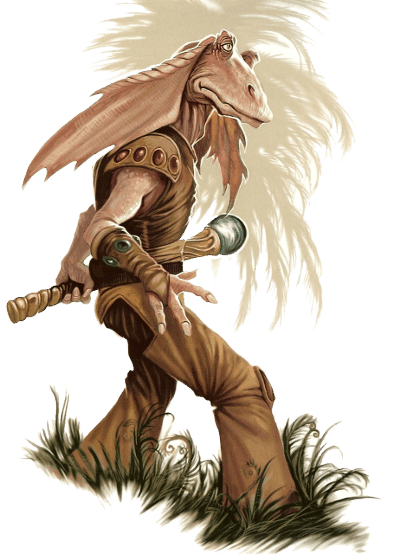
\includegraphics[width=6cm]{img/personnages/races/gungan.png}
	\vspace{-12\baselineskip}

	\begin{flushright}
		\begin{tabular}{ l l }
			\textbf{Type} 			& Amphibien \\
		   	\textbf{Planète} 		& Naboo \\
		   	\textbf{Langage} 		& Gunganese \\
		   	\textbf{Orientation} 	& Lumineux \\
		\end{tabular}
	\end{flushright}

	\vspace{7\baselineskip}
\end{samepage}

Natifs de la planète Naboo, les Gungans vivent dans des cités sous-marines. La physiologie d’un Gungan est de type humanoïde, quoique plus grand et plus fin qu’un Humain. Les Gungans possèdent de longues oreilles tombantes, des narines souples et des membranes rétractiles protégeant les yeux lors de leur déplacement aquatique. Leurs articulations sont libres et les ligaments très souples, permettant aux amphibiens de nager avec aisance sous l’eau.

\begin{description}[align=left]
\item [Aquatique] 					% CAP +2 +1
		Les gungans vivent dans les grandes étendues d’eau de Naboo, ils ne peuvent se noyer. Ils se déplacent sous l’eau beaucoup plus vite que n’importe qu’elle autre espèce.\\
		\emph{d6 Natation}\\
		\emph{Allure sous l’eau = d Natation}
		
\item [Mollusque] 					% CAP +3
		Leurs articulations sont libres et les ligaments très souples, permettant aux amphibiens de nager avec aisance sous l’eau. Cette souplesse leur permet de se faufiler dans des endroits étroits et d’esquiver les attaques avec plus de réussite.\\
		\emph{Atout Esquive}

\item [Craint la chaleur] 			% CAP -2
		Leur physiologie aquatique rend les Gungans plus sensible aux fortes températures et à la sécheresse d’un climat.\\
		\emph{-4 pour résister à la chaleur}

\item [Langue bien pendue] 			% CAP -1
		Les Gungans passent le plus clair de leur temps à parler, de tout et n’importe quoi, surtout n’importe quoi. Néanmoins il arrive que la parole dépasse leur pensées et qu’ils livrent des secrets qu’ils n’auraient pas du livrer.\\
		\emph{Handicap Bavard}

\item [Maladroit] 					% CAP -1
		La culture Gungan est une relation poussée entre la nature et l’individu. Ils essaient de ne pas utiliser la technologie, se servant de ce que la Nature propose. Ils n’ont que peu l’habitude de la technologie conventionnelle et évitent de la manipuler sous peine de détraquer tout ce qu’ils touchent.\\
		\emph{Handicap Deux mains gauches}
\end{description}